%\section{\texorpdfstring{Polynomial Hierarchy cont}{Polynomial Hierarchy cont}}
%\vspace{5mm}
%\large

%\subsection{Tutorial}

%\begin{exercise}
%	\begin{enumerate}[label=\alph*)]
%		\item $\exists \TP = \TNP$.
%		\item $\forall \TP = co-\TNP$.
%		\item $\forall k > 0: \exists \Sigma_k = \Sigma_k$
%		\item $\forall k > 0: \forall \Pi_k = \Pi_k$
%		\item $\exists \Pi_k = \Sigma_{k + 1}$
%		\item $\forall \Sigma_k = \Pi_{k + 1}$
%	\end{enumerate}
%\end{exercise}

\subsection{PH collapse}

\begin{theorem}[Polynomial hierarchy collapse at level k]\label{ph_collapse}
	if $\Sigma_k = \Pi_k$ for some $k > 0$ then
	\[ \forall j \geq 0: \Sigma_{k + j} = \Pi_{k + j} = \Sigma_k \]
\end{theorem}
\begin{proof}
	By induction on j. For 0 is true by assumption.

	Induction step:
	\[ \Sigma_{k + j + 1} \xlongequal{\cref{polyn_q}\ c)} \exists \Pi_{k + j} \xlongequal{I.H.} \exists \Sigma_{k + j} \]
	By \cref{polyn_q} c)
	\[ \exists \Sigma_{k + j} = \Sigma_{k + j} \]
	By I.H. again
	\[ \Sigma_{k + j} = \Sigma_k \]

	Similarly for $\Pi_{k + j + 1}$.
	\[ \Pi_{k + j + 1} \xlongequal{\cref{polyn_q}\ f)} \forall \Sigma_{k + j} \xlongequal{I.H.} \forall \Pi_{k + j} \xlongequal{I.H.} \Sigma_k \]
\end{proof}

\begin{theorem}[PH not collapse]
	Either $\forall k: \Sigma_k \subset \Sigma_{k + 1}$ or PH collapses.
\end{theorem}
\begin{proof}
	Assume
	\[ \Sigma_k = \Sigma_{k + 1} \]
	We know
	\[ \Sigma_{k + 1} = \TNP(\Sigma_{k}) = \TNP(\Pi_k) \supset \Pi_k \]
	Implies by assumption
	\[ \Pi_k \subseteq \Sigma_k \Rightarrow \Sigma_k = \Pi_k \]
	Then by \cref{ph_collapse} PH collapses after $k$.

	In particular for $k = 0$ we get
	\[ \TP = \TNP \Rightarrow PH = \TP \]
\end{proof}

\begin{consequence}
	\[ \text{If}\ \exists k \in \N: \TP = \Sigma_0 \subset \Sigma_k \Rightarrow \TP \subset \TNP \]
\end{consequence}
\begin{proof}
	By reversing previous condition.
\end{proof}

\begin{definition}[PSPACE-complete]
	$L$ is PSPACE-complete if: \\
	$L \in PSPACE$ and\\
	$\forall L_a \in PSPACE: L_a$ is poly time reducible to $L$.

	Note that we use Time reducibility for Space class.
\end{definition}

\begin{lemma}[$PH = \Sigma_k$]\label{ph_col_lemma}
	Let $L$ be $PS$-complete and $L \in \Sigma_k$ then $PH = \Sigma_k$.
\end{lemma}
\begin{proof}
	Take $L_2 \in PS$ arbitrary, then by the polynomial reduction
	\[ \exists DTM\ M_d: x \in L_2 \iff M_d(x) \in L \]
	$M_d$ is a transducer.

	Also there is acceptor
	\[ \exists NTM\ M_n, \exists D \in \Sigma_{k - 1}: L = L(M_n, D) \]
	Then we construct new NTM by concatenation of $M_d$ and $M_n$.

	% todo join 2 proofs, predn 5 od 33:00
	\[ L_2 \in PS \]
	Therefore
	\[ PS \subseteq \Sigma_k \]
	We already know that
	\[ PH \subseteq PS \]
	Therefore
	\[ PH = \Sigma_k \]
\end{proof}

\begin{consequence}
	if $PH = PS$ then
	\[ \exists k \in \N: PH = \Sigma_k \]

	Assuming that $\exists L \in PS$-complete.

	Which implies, that if PH grows infinitely and no PS-complete is in PH.
	Then $PS \setminus PH$ contains all $PS$-complete languages.
\end{consequence}
\begin{proof}
	We take L, by $PH = PS$
	\[ \exists k: L \in \Sigma_k \]
	then by \cref{ph_col_lemma}
	\[ PH = PS \]
\end{proof}

\section{\texorpdfstring{PS-complete lang}{PS-complete lang}}
\vspace{5mm}
\large

\begin{definition}[QBF - quantifiable boolean formula]
	%todo predn 5 od 50:00
	\begin{enumerate}
		\item if $x$ is a variable then $x$ is a QBF and $x$ is a \emph{free} variable
		\item if $E_1, E_2$ are QBF then
			\[ \neg E_1, (E_1) \land (E_2), (E_1) \lor (E_2) \]
			are also QBFs.

			And the status of variables (free/bounded) does not change.
		\item if $E$ is a QBF then
			\[ \exists x (E), \forall x (E) \]
			are also QBFs. And all ocurrences of $x$ become bounded.
			Status of other variables does not change.
	\end{enumerate}
\end{definition}

\begin{definition}[QBF problem]
	QBF problem (language).

	Input: QBF $F$ with no free variables.

	Question: $F = 1$??
\end{definition}

How do we evaluate QBF with no free variables?
\begin{itemize}
	\item $ \exists x (E) \iff E_0 \lor E_1$
	\item $ \forall x (E) \iff E_0 \land E_1$
\end{itemize}
Where $E_0$ is formula where every occurrence of $x$ is replaced by $0$.
Similarly $E_1$.

\begin{example}
	\[ \forall x (\forall x (\exists y (x \lor y)) \land \neg x) \]
	by rules above
	\[ (\forall x (\exists y (x \lor y)) \land \neg 0) \land (\forall x (\exists y (x \lor y)) \land \neg 1) \]
\end{example}

\begin{note}
	SAT - language of satisfiable CNFs.
	We can think of it as
	\[ \exists x_1 \exists x_2 \ldots \exists x_n (F(x_1, x_2, \ldots, x_n)) \]
	Therefore SAT is a special case of QBF.
\end{note}

\begin{theorem}[QBF $\in$ PS]
	QBF $\in$ PS.
\end{theorem}
\begin{proof}
	We construct DTM to evaluate QBF without free variables as following
	\begin{itemize}
		\item $\neg(E) \to$ evaluate E and negate all results
		\item $(E_0) \lor (E_1) \to $ evaluate $E_0$, $E_1$ then by disjunction
		\item $(E_0) \land (E_1) \to $ evaluate $E_0$, $E_1$ then by conjunction
		\item $\exists (E) \to$ compute $E_0, E_1$, then compute $E_0 \lor E_1$
		\item $\forall(E) \to$ compute $E_0, E_1$, then compute $E_0 \land E_1$
	\end{itemize}

	We have at most $n$ operators.
	We get binary tree that evaluates the formula.
	Where every branch is bounded by total length of initial formula.

	$\bigO(n^2)$ is enough space for evaluation.
\end{proof}

\begin{example}
	\[ F = \vee_{1 \leq j \leq n} (x_i \to y_i) = \vee_{1 \leq j \leq n} (\neg x_i \lor y_j)\]
	Can be viewed as bipartite graph.

	Claim: The resulting formula is shortest CNF representing $F$.
	By the completness of resolution.
	Length changed to $\Theta(n^2)$.

	Now 2nd formula
	\[ H = (\exists z) [(\wedge_{1 \leq i \leq n}(x_i \to z)) \land (\wedge_{1 \leq j \leq n} (z \to y_j))] \]
	$H$ is an encoding of $F$ with auxiliary variables.
	Can be viewed as bipartite graph but with single node in between parts.
	%todo image predn 5 od 1:19:00

	However, $H$ is shorter since it is $\Theta(n)$.
\end{example}
\begin{proof}
	As every $x$ implies every $y$ models of $F$ are:
	\[ (0, 0, 0, \ldots, *, * \ldots, *) \cup (*, * \ldots, *, 1, 1, \ldots, 1)\]
	Where $*$ represents arbitrary value.

	If we rewrite $H$ and substitute $0 \lor 1$ for $z$ we get:
	\[ [(\wedge_{1 \leq i \leq n}(x_i \to 0)) \land (\wedge_{1 \leq j \leq n}(0 \to y_j))] \lor [(\wedge_{1 \leq i \leq n}(x_i \to 1)) \land (\wedge_{1 \leq j \leq n}(1 \to y_j))]\]
	Therefore models are the same.
\end{proof}

\begin{note}
	Trick with auxiliary variables is used, if we have a requirement of only one $x_i$ to be 1.
	Which can be represented by formula:
	\[ \wedge_{1 \leq i,j \leq n}(x_i \lor \neg x_j) \]
	Which is $\Theta(n^2)$ and auxiliary variable makes it linear.
\end{note}

\begin{theorem}[QBF is PS-hard]
	QBF is PS-hard (sketch).
\end{theorem}
\begin{proof}
	Every $L \in PS$ arbitrary can be reduces to QBF in poly time.

	By the definition of PS
	\[ \exists DTM\ M: L = L(M), \exists p(n)\ \text{M accepts L in space}\ p(n)\]

	We have $2^{c_m p(n)}$ configurations of M and every configuration can be encoded by string of length
	\[ c_m p(n) = m(n) := m \]
	We assume, that there is only 1 accepting configuration.

	$x \in L \iff \exists $ path of length $m$ in \emph{configuration graph} from $C_0 \to C{acc}$.
	Use similar algorithm as in Savic theorem \cref{savic}, but encode computation in QBF.

	Notation, where $\varphi$ is an encoding of allowed transition in Cook-Levin theorem.
	We construct QBF $\psi$.
	\begin{itemize}
		\item $ \psi_0(C, C^{\prime}) = 1 \iff \varphi_m(C, C^{\prime})$ is satisfiable
		\item $ \psi_i(C, C^{\prime}) = 1 \iff $ there exists path $C \to C^{\prime}$ of length $2^i$
		\item $ \psi_m(C_0, C_{acc}) = 1 \iff x \in L$
	\end{itemize}

	Obvious idea that would not work
	\[ \psi_i(C, C^{\prime}) = \exists C_{int} (\psi_i(C, C_{int}) \land \psi_i(C_{int}, C^{\prime})) \]
	Since every such change doubles size of the formula, we end up with
	\[ |\psi_m| \in \Omega(2^m p(n)) \]

	Main idea
	\[ \psi_i(C, C^{\prime}) = \exists C_{int} \forall D_1, D_2 [(D_1 = C \land D_2 = C^{\prime}) \lor (D_1 = C_{int} \land D_2 = C^{\prime})] \Rightarrow \psi(D_1, D_2) \]
	Formally, implication could be replaced by $\neg x \lor y$.
	Now
	\[ |\psi_i| = |\psi_{i - 1}| + \bigO(m) \]
	Therefore
	\[ |\psi_m| = \bigO(m^2) \]

	Also, going from $\psi_{i - 1} \to \psi_{i}$ we need 1 existential, 1 universal quantifier.
	In the end, $\psi_m$ has $m$ pairs of alternating existential and universal quantifiers.

	Therefore $QBF \in \Sigma_m$.
\end{proof}

\subsection{P-completeness}

\begin{note}
	If we use polynomial time reducibility, almost all languages(except trivial: empty and all words) are $\TP$-complete.

	Therefore we use a different reducibility.
\end{note}

\begin{definition}[log-space reducibility]\label{log_red}
	A is \emph{log-space} reducible to B if $\exists$ DTM transducer M that works in log space (excluding input and output tape).
	Such that $x \in A \iff M(x) \in B $.
\end{definition}

\begin{definition}[$\TP$-complete]
	L is $\TP$-complete $\iff L \in \TP \land \forall A \in \TP A$ is log-space reducible to L.
\end{definition}

\begin{theorem}[P-complete vs LOG]\label{p_comp_log}
	Let $L$ be $\TP$-complete and $L \in LOG = DS(\log(n)) \Rightarrow \TP = LOG$.
\end{theorem}
\begin{proof}
	Since $c_n^{\log n} = (2^{\log n})^{\log c_n} = n^{\log c_n}$.
	\[ LOG \subseteq \TP \]
	We want
	\[ \TP \subseteq LOG \]

	Let $B \in \TP$ arbitrary, we need log-space acceptor for B $\Rightarrow B \in LOG$.
	From $L$ is $\TP$-complete $\Rightarrow \exists$ log-space DTM $M_L: x \in B \iff M_L(x) \in L$.
	From $L \in LOG \Rightarrow \exists $ log-space DTM acceptor $M_{log}: L = L(M_{log}) $.

	We cannot simply concatenate 2 machines, as output tape of the first machine $M_L$ becomes work tape of the 2nd.
	Output tape is not guaranteed to be log-space.
	Let $Y$ be the output of $M_L$
	\[ |Y| \leq 2^{c_M \log n} = n^{c_M} \]

	Idea: keep just current symbol on output of $M_L$ and the position.
	Then start the next step of $M_{log}$.
	Then restart $M_L$ and discard output with position $ < i$.
	Repeat.

	Works, because we do not worry about Time, but space.

	We need 2 counters $i, j \in \{ 1, \ldots, |Y| \}$.
	Which require
	\[ \log(n^c) = c \log n \]

	Where $i$ keeps the position, updates with every move of the head.
	$j$ is reset to $0$ and is incremented with every symbol $M_{log}$ outputs.

	Symbols are discarded until $i = j$.
	%One counter is incremented with write on output tape, other counter keeps position on the output tape.
	%while(work)
	%{
	%	for(j = 0; j < i; ++j)
	%	{
	%		if(
	%	}
	%}

	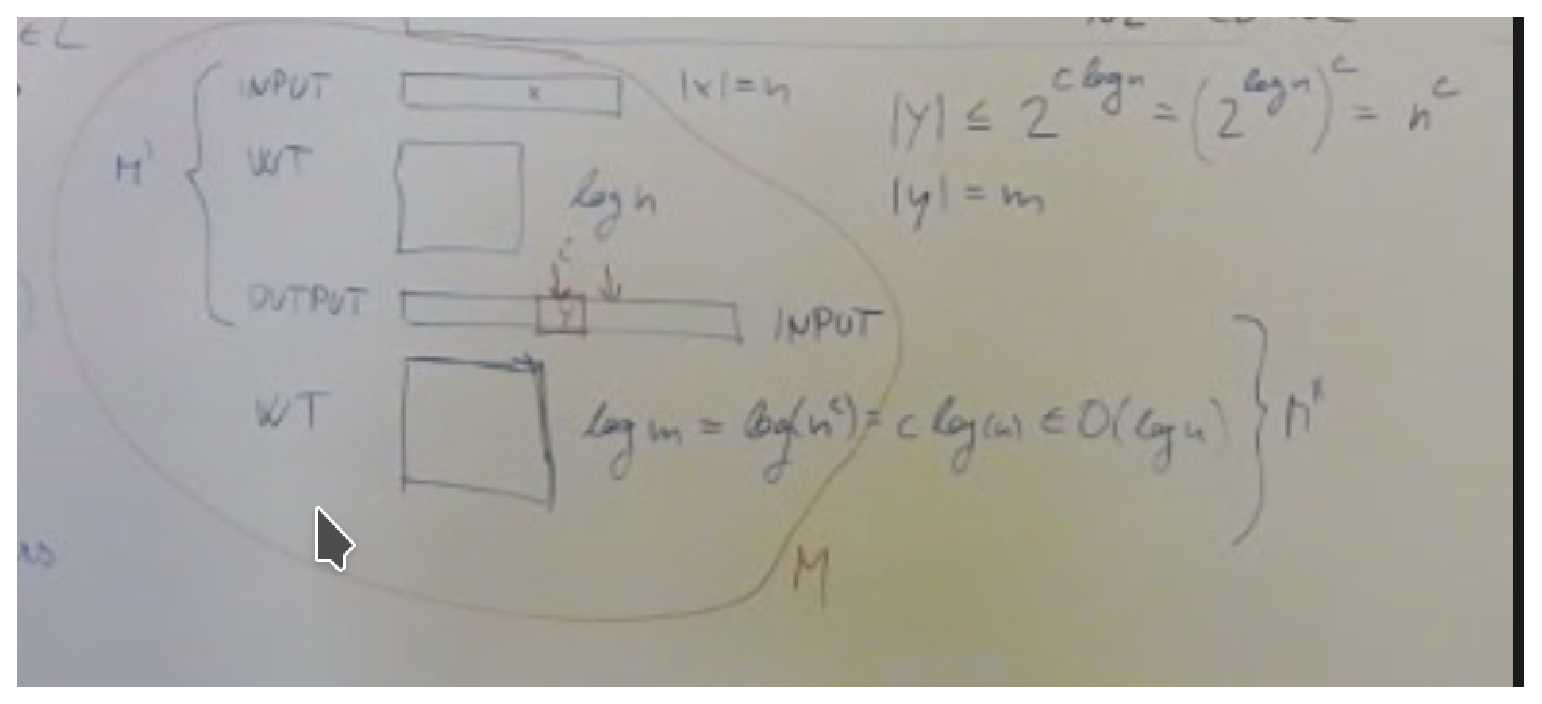
\includegraphics[scale=0.4]{p_nlog.eps}
\end{proof}

\begin{consequence}
	Let $L$ be $\TP$-complete and $L \in NLOG = NS(\log(n)) \Rightarrow \TP = NL$.

	Proof is same, but acceptor is non deterministic.
\end{consequence}

Q: what if we use log-space reducibility in $\TNP$-complete definition?
This is stricter, since if we can reduce in log-space, we can also reduce in polynomial time (by time and space comparison with $2^n$).

\subsection{$NL = co-NL$ by Szelepcsenyi-Immerman}
% 6th lecture

\begin{theorem}[Szelepcsenyi-Immerman(1988)]
	\[NL = co-NL \]
\end{theorem}
\begin{proof}
	Similar proof as in case $L \in \TNP$-complete $\land L \in co-\TNP$.
	But the reducibility is again log space \cref{log_red}.

	Assume, $L \in NL$-complete.
	Let $L_a \in NL$ be arbitrary.

	Let $M_{log}$ be a log space transducer, $M$ be acceptor for $co-L$.

	Then $M_{log} + M$ is an acceptor for $co-L_a$.

	Output of the transducer can be quite large.
	Which then becomes working tape for acceptor.
	Similarly, as in previous theorem \cref{p_comp_log} output of the transducer is added character by character.

	Let the desirable language be
	\[ L = PATH = \{ (G, s, t)|\ \text{G is an undirected graph in which}\ \exists Path(s, t) \} \]
	Graph can be encoded by the following:
	\begin{itemize}
		\item for $n$ vertices $\log n$ counter is enough.
		\item for each vertex we store list of neighbors.
	\end{itemize}

	Easy to see, that PATH $\in \TP$, since BFS, DFS can solve problem in poly time.

	PATH $\in LOG$ is an open question.
	However, with NTS log space is enough since we can try all paths with size $n$ by picking the next neighbor randomly.
	In each step it is sufficient to remember code of the current vertex and path size counter on separate tapes.
	Both of them are of size $\bigO(\log n)$.

	The algorithm:
	\begin{enumerate}
		\item vertex curr $= s; counter = 0$;
		\item while($counter < n$)\{
		\item pick neighbor U at random; if($U = t$) accept;
		\item $curr = U$;
		\item \}
		\item reject.
	\end{enumerate}

	To show that PATH is $NL$-hard, we will treat the graph as the configuration graph.
	And the $Path(s, t)$ will be a path from $C_0$ to $C_{accept}$.
	WLOG there is only one $C_{accept}$ configuration.

	Let $L_a \in NL$ be arbitrary, therefore $\exists$ log space acceptor $M: L_a = L(M)$.

	Transducer $M_{log}$ encodes the configuration graph of $L_a$.

	Code of the acceptor is not a problem, as size of $M$ does not depend on the input.
	Transition table if $M$ is embedded in the control unit.

	Space needed for 1 configuration of $M$ is $\bigO(\log n)$.
	As the work tape is bounded by the assumption, and for the position of the head $\bigO(\log n)$ is also enough.

	The last step is to prove co-PATH $\in NL$.
	Algorithm is the following:
	\begin{itemize}
		\item count vertices reachable from $s$ in G.
		\item count vertices reachable from $s$ in $G \setminus \{t\}$.
		\item if equal - accept.
	\end{itemize}

	There is no need to generate encoding of graph $G \setminus \{t\}$, since $t$ is part of input and we can ignore it by single "if".

	How to count reachable vertices? The number is bounded by $n$ therefore, $\bigO(\log n)$ space is enough.

	\begin{definition}[$R_i$]
		\[ R_i = \{ u |\ u\ \text{is reachable from}\ s\ \text{by path length}\ \leq i \} \]
		Also
		\[ R_i = R_{i - 1} \cup \{ a |\ \exists b \in R_{i - 1}: (a, b) \in E(G) \} \]
	\end{definition}

	We want to compute $|R_n|$.
	To do so, we compute non-deterministically compute $|R_0|, |R_1|, \ldots, |R_n|$.
	At each step, we remember only the last number.
	Algorithm to compute $R_i$:
	% todo rewrite, extremely messy
	\begin{enumerate}
		\item $|R_0| = 1$;
		\item guess $0 \leq g \leq n$ and verify:
			\begin{enumerate}
				\item $g \geq |R_i|$\\
					Generate non-deterministically all subsets $V \subseteq V(G)$ of vertices of size $g$.
					Vertices are ordered by increasing number of their codes.
					Check whether $\forall v \in V: \exists Path(s, v): |Path(s, v)| = g$.
				\item $g \leq |R_i|$.\\
					Is equivalent to check
					\[ |V \setminus R_i| \geq n - g \]
					Algorithm:
					% todo rewrite as procedure
					\begin{enumerate}
						\item non deterministically generate $V_t \subseteq V(G): |V_t| = (n - g)$ vertices.
						\item $\forall a \in V_t$ check $a \in V(G) \setminus R_i$.
						\item generate $V_r \subseteq V(G): |V_r| = |R_{i - 1}|$ non deterministically: select $|R_{i - 1}|$ vertices and check $Path(s, a): |Path(s, a)| = i - 1$.
						\item $\forall b \in V_r$ check $a \ne b \land (b, a) \notin E(G)$.
					\end{enumerate}
			\end{enumerate}
	\end{enumerate}

	Required space is again $\bigO(\log n)$ as in each step algorithm stores constant number of vertices.
\end{proof}
